\documentclass[aps,pre,reprint,floatfix,superscriptaddress,nofootinbib]{revtex4-2}
\usepackage{amsmath,amssymb,amsthm,graphicx,booktabs,array,hyperref,microtype}
\hypersetup{colorlinks=true,linkcolor=black,citecolor=blue,urlcolor=black}\setlength{\emergencystretch}{2em}
\newcommand{\dmin}{d_{\min}}\newcommand{\R}{\mathbb R}\newcommand{\tr}{\operatorname{tr}}
\DeclareFontShape{OT1}{cmss}{m}{n}{<->cmss10}{}
\newtheorem{theorem}{Theorem}
\begin{document}
\title{Time-reversal inference with uncertain observation channels}
\author{Dev D. Goyal}
\email{dvgyl@outlook.com}
\thanks{ORCID: 0009-0009-9132-744X}
\affiliation{Independent researcher}
\date{7 October 2026}
\begin{abstract}
When one measured signal tends to follow another, the time order can come from the physical source or from unequal sensor responses. We ask when a finite recording can distinguish these explanations. A reversible source has the same statistical behavior forward and backward in time. We study stationary Gaussian models, with time-independent statistical rules and joint normal distributions. With unrestricted source frequencies and sensor delays, we construct reversible sources that give exactly the same finite-record probabilities as asymmetric sources. Suitable delays can be arbitrarily small if sampling makes distinct continuous-time frequencies indistinguishable. Useful tests therefore need additional information. Calibration with a known input bounds the asymmetry that two sensors can create. With three channels, a product of pairwise frequency measurements cancels detector phase, the part that describes relative timing. This cancellation requires each response to act on its own sampled source channel. Both tests need a bound on dependence across the complete record. The frequency-based test also needs a bound on correlations beyond the retained time separations. With these bounds, the tests control the probability of wrongly rejecting a reversible-source explanation. A simulated Brownian gyrator describes a trapped particle subject to thermal fluctuations. At equal bath temperatures, unequal sensors lead a raw block-bootstrap test to detect recorded asymmetry in 397 of 400 records of length $N=524289$. The calibrated source test rejects none, while detecting all 200 records at a fourfold bath-temperature ratio at the same length. The raw test concerns the recording. Attributing its equilibrium detections to the source would be wrong here. Correlation and uncertainty about its decay can require long recordings. Finally, identical sampled rotations can have unboundedly different entropy-production rates, a thermodynamic measure of irreversibility. Detector information can support a source test, but cannot recover motion hidden between samples.
\end{abstract}
\maketitle

\begin{figure*}[t]
\centering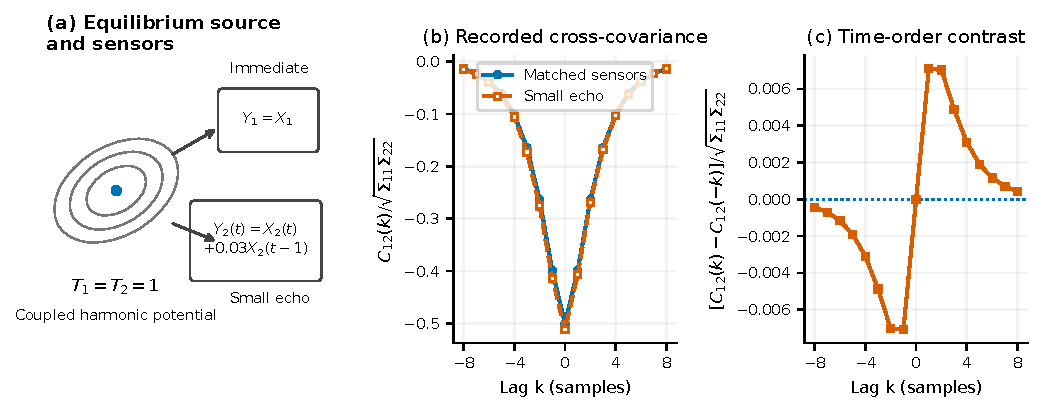
\includegraphics[width=\textwidth]{figures/equilibrium_sensor_example.pdf}
\caption{Unequal sensors can make equilibrium fluctuations appear to have a preferred time order. Cross-covariance measures how the two signals vary together at a given time separation, or lag. The Brownian model gives a symmetric curve with matched responses and an asymmetric curve when channel 2 includes a $0.03$ one-sample echo. Both curves use the same source-variance normalization. The odd part is half the difference between a cross-covariance curve and its time-reversed version. It isolates the asymmetry. Curves are exact model calculations, not sample estimates. The source, sampling interval, and marginal temperatures are unchanged.}\label{fig:sensor-example}
\end{figure*}

\section{Introduction}
A measured time order need not come from the physical system. Consider two sensors observing coupled fluctuations. One responds immediately, while the other averages recent values. The second signal can then follow the first even though the source has no statistical preference for forward over backward time. Such a source is called reversible. Figure~\ref{fig:sensor-example} shows this effect for a Brownian particle at thermal equilibrium, with both coordinates coupled to heat baths at the same temperature. A longer record resolves the time difference, or lag, more clearly, but cannot by itself identify its physical origin.

Researchers use time asymmetry to detect nonequilibrium activity~\cite{gonzalezarea2019,ohgaasymmetry2023,cerasolispectra2022,seara,gnesotto2018}. A cross-correlation measures how two signals vary together at a chosen lag. It does not establish that one causes the other. A cross spectrum expresses this relation by frequency. Its phase describes relative timing at that frequency. Sensor filters and unequal acquisition times alter that timing~\cite{tongzhang,bhandari2026}. In multichannel fluorescence imaging, emission-filter switching delays acquisitions at different wavelengths~\cite{stehbens2012}. In optical trapping, photodiodes and electronics can suppress fast changes in the measured position~\cite{bergsorensen2004}. These instrument effects matter when testing whether active biological systems have balanced forward and reverse transitions, called detailed balance~\cite{battle2016}. Mistaking a sensor lag for source dynamics can lead to a false claim of physical driving or energy dissipation.

Related methods estimate entropy production in actomyosin, a network of interacting actin and myosin proteins~\cite{seara2018}. Other methods bound dissipation from fluctuating currents~\cite{li2019}. Cycling frequencies measure circulation in the space of observed fluctuations~\cite{mura2018,gradziuk2019}. These approaches use different observables and assumptions, but each links measured motion to physical activity.

Our equilibrium simulation makes this distinction concrete. A raw bootstrap test, which estimates uncertainty by resampling blocks of the recording, detects asymmetry in $87/400$ short records and $397/400$ long records. The source stays reversible throughout. The increasing evidence concerns the recorded signal, so a source interpretation requires additional detector information.

What must be known about the detectors, and how much data are needed, before an asymmetric recording rules out every allowed reversible source? We answer this question for stationary Gaussian sources and linear observation channels. Stationarity means that statistical behavior does not change when the whole observation period shifts in time. Gaussian models use joint normal distributions. Their means and covariances determine those distributions completely. Covariance measures how fluctuations vary together, including their scale. A linear sensor records a weighted sum of source values, possibly with added error. These restrictions make it possible to give exact probability bounds.

The first result states what data alone cannot resolve. With unrestricted spectra and channel delays, every nonsingular finite stationary Gaussian law admits a reversible-source explanation. Here a law specifies the joint probabilities of all values in the record. Integer delays can move the distinguishing covariance beyond the observed lags. Sampling can also make different continuous-time frequencies indistinguishable, an effect called aliasing. If those frequencies are unrestricted, aliasing permits the same ambiguity with suitable delays as small as desired. Thus a useful test must exclude some observation mechanisms through physical information.

We then give two routes to a source test. Calibration measures sensor responses using a known input and bounds the asymmetry that two detectors can create. With a third channel, pairwise spectral phases can be combined around a triangle so that each detector phase cancels. This operation is called closure phase and requires the sampled response model stated below. Both routes need bounds on temporal dependence because correlated samples give less information than independent samples. We quantify the resulting recording cost and show how to estimate correlation persistence from a noiseless reference. The final example returns to aliasing. Sampling can hide circulation and therefore cannot determine continuous-time entropy production, the thermodynamic rate associated with irreversibility.

Sections~\ref{sec:observation} and~\ref{sec:ambiguity} define the observation problem and prove its unrestricted ambiguity. Sections~\ref{sec:calibrated} and~\ref{sec:main-cycle} develop the two tests together with their physical results. Section~\ref{sec:cost} treats recording length and unknown persistence. Section~\ref{sec:sampling} then separates sampled inference from the dynamics between observations.



\section{The source and its observation channels}\label{sec:observation}
For the equilibrium example, the relevant symmetry concerns the particle before its signals pass through the sensors. Covariance measures how two fluctuations vary together, including their scale. Let $C^X_{ij}(k)$ be the covariance of source channels $i$ and $j$ at a time separation, or lag, $k$. Because means and covariances determine the Gaussian law, their symmetry can establish reversibility. After subtraction of the mean, a stationary Gaussian process whose coordinates have a common time-reversal parity satisfies
\[
 \text{reversibility}\quad\Longleftrightarrow\quad
 C^X_{ij}(k)=C^X_{ij}(-k).
\]
The equality must hold for every channel pair and lag. It makes the full Gaussian law invariant under reversal, since the mean and covariance determine that law. Equivalently, the source cross-spectral measure is real. The common-parity condition includes position coordinates, which keep their signs under reversal, and separately velocity coordinates, which change their signs. A mixture of positions and velocities requires parity signs in the covariance criterion and is outside the convention used here.

The spectrum expresses the same covariance relations by frequency, where a detector timing change becomes a phase factor. A linear sensor records a weighted sum of source values. This operation changes both the amplitude and timing of the signal. Write its transfer function as $H_i(\omega)$ for channel $i$ and frequency $\omega$. A pure delay has response $e^{-id_i\omega}$, while the echo in Fig.~\ref{fig:sensor-example} has response $1+0.03e^{-i\omega}$. If $\mu$ is the matrix spectral measure of the source, the recorded spectral measure is
\begin{equation}
 F=D_H\mu D_H^*+F_E,\qquad D_H=\operatorname{diag}(H_i).
 \label{eq:main-model}
\end{equation}
The star denotes conjugate transpose. The source and errors are jointly Gaussian and stationary. Errors are uncorrelated with the source and between channels at every lag, so their spectral measure $F_E$ is diagonal. Unknown constant means are allowed. For $i\ne j$, Eq.~\eqref{eq:main-model} multiplies the source cross spectrum by $H_i\overline H_j$. Its phase can therefore change even when the source spectrum is real.

We use $C_{ij}(k)=\operatorname{Cov}\{Y_i(t+k),Y_j(t)\}=\int e^{ik\omega}F_{ij}(d\omega)$ for the recorded covariance. Discrete-time densities use $d\omega/(2\pi)$ on $[-\pi,\pi]$. Spectral measures also allow contributions concentrated at individual frequencies. Equation~\eqref{eq:main-model} describes filters acting on the sampled source sequences. Filtering in continuous time before sampling does not always give this factorization. Distinct continuous frequencies can become one sampled frequency while retaining different detector phases. This aliasing will matter both for the ambiguity result and for the interpretation of phase cancellation.

\subsection{Equilibrium and driving in a trapped particle}
We use a Brownian gyrator to connect the statistical symmetry to a physical source~\cite{filliger2007,cerasolispectra2022,argun2017}. A particle moves in a two-dimensional harmonic trap. The restoring force couples its coordinates, and each coordinate receives random forcing from a heat bath. In the overdamped limit, where inertia is neglected, the dimensionless dynamics are
\begin{equation}
 \begin{gathered}
 dX=-AX\,dt+\sqrt{2D}\,dW_t,\\
 A=\begin{pmatrix}1&1/2\\1/2&1\end{pmatrix},\quad
 D=\operatorname{diag}(T_1,T_2).
 \end{gathered}
 \label{eq:ou-model}
\end{equation}
Here $dW_t$ supplies the random forcing, and the stationary covariance satisfies $A\Sigma+\Sigma A^{\mathsf T}=2D$. Equal bath temperatures give equilibrium. Unequal temperatures produce a circulating stationary probability current: trajectories favor one direction around the trap although the position distribution stays constant. We sample at interval one and then apply $H_1=1$, $H_2=1+0.03e^{-i\omega}$. The equilibrium curve in Fig.~\ref{fig:sensor-example} therefore isolates the effect of unequal detectors within Eq.~\eqref{eq:main-model}. The same source model with unequal temperatures will test whether detector information permits detection of physical driving.

Throughout the paper, the null hypothesis is a reversible source observed through the allowed channels. A test must control the probability of rejecting this explanation whenever it is true. Failure to reject does not establish reversibility. We also distinguish nonrejection from abstention: a test abstains when a required bound or numerical comparison is unavailable. A source outside the null class is an alternative. Its rejection probability is the detection probability, or power. All records, including abstentions, remain in the denominators of the reported rejection fractions. Table~\ref{tab:notation} in Methods collects the main symbols.

\section{What a finite recording cannot decide}\label{sec:ambiguity}
The equilibrium example suggests a possible remedy: collect enough data to resolve the source and detector contributions separately. Without restrictions on the source or detectors, this remedy fails. A finite record contains only finitely many covariance lags. A delayed reversible source can agree with an asymmetric source at every retained lag and differ only outside the record.

Consider two explanations for the same two-time record. In the first, the source is asymmetric and the sensors add no delay. In the second, the source is reversible and one sensor delays it. Each channel separately has variance one and no covariance between distinct times, called a unit white marginal spectrum. The first explanation has cross spectrum
\[
 F^A_{12}=\tfrac1{10}+\tfrac15e^{-i\omega}.
\]
A reversible source with $S^R_{12}=\tfrac15+\tfrac15\cos\omega$, observed after delaying channel 1 by one sample, instead gives
\[
 F^R_{12}=e^{-i\omega}S^R_{12}
 =\tfrac1{10}+\tfrac15e^{-i\omega}+\tfrac1{10}e^{-2i\omega}.
\]
The spectral eigenvalues are at least $7/10$ and $3/5$, respectively, so both constructions are positive and define valid Gaussian processes. Their cross-covariances are
\[
\begin{array}{c|ccccc}
 k&-2&-1&0&1&2\\\hline
 C^A_{12}(k)&0&0&1/10&1/5&0\\
 C^R_{12}(k)&0&0&1/10&1/5&1/10
\end{array}
\]
A two-time record sees only lags $-1,0,1$, the middle three columns. Its complete covariance, and hence its Gaussian law, agrees under both explanations. The extra term in the second spectrum changes only the last column shown. Lag two would distinguish the explanations, but is absent from that record.


The following result extends that construction from a two-time example to every finite stationary Gaussian law with positive-definite covariance. Positive definiteness excludes an exact linear constraint between recorded fluctuations. The constructed sources have finite dependence: their covariances vanish beyond a finite lag.
\begin{theorem}[Finite-law ambiguity]\label{thm:main-finite-law}
Fix a positive record length and a nonempty finite collection of stationary Gaussian record laws with positive-definite covariance matrices and the same number of channels. One vector of nonnegative integer channel delays gives a reversible Gaussian source representation for every law in the collection. Each source has a strictly positive matrix trigonometric polynomial spectral density and finite dependence. The sources preserve the channel means and variances. No observation error is needed.
\end{theorem}
Thus even the exact finite joint distribution cannot exclude a reversible source in this unrestricted class. A test with false-rejection probability at most $\alpha$ throughout that class has detection probability at most $\alpha$ against every nonsingular finite stationary Gaussian alternative. The proof constructs a positive reversible spectrum, then corrects the retained moments exactly (Supplemental Material, abbreviated SM, Sec.~S1, Theorem~S1 and Proposition~S1). An approximate covariance match would not suffice.

For two channels and $N\ge2$, generic retained covariances require integer relative delay at least $N-1$. The exceptional records satisfy $C_{12}(\Delta-1)=C_{12}(\Delta+1)$ for an integer $|\Delta|\le N-2$. The minimum scale is attainable under an additional covariance condition (SM Sec.~S1.2). The source and delays can depend on record length; the result concerns a fixed finite law, not one representation valid at all lengths.

Large delays are not the only source of ambiguity. Suitable prescribed real delays, whose nonreference relative delays are rationally independent with the sampling interval, can be arbitrarily small when continuous frequencies are unrestricted. This means that no nonzero integer combination of those delays and the interval is zero. Aliased frequencies then supply the required channel phases (SM Sec.~S2, Theorem~S3 and Corollary~S2). A spectral envelope instead bounds the effect of small skew (Proposition~S3). Bandwidth control therefore matters as well as timing accuracy~\cite{hansenSargent1983,parratobar,rutten}. The next two sections restrict the ambiguity through response calibration or phase cancellation, together with quantitative covariance bounds.

\section{Two channels with response calibration}\label{sec:calibrated}
Calibration makes a source claim testable by limiting how much asymmetry the detectors can explain. A known test input bounds their relative phase, which then bounds their contribution to the observed asymmetry. Variance measures the size of fluctuations within one channel. For aligned recordings with variances $v_1,v_2$, consider
\begin{equation}
 \kappa=C_{12}(1)-C_{12}(-1).
 \label{eq:main-contrast}
\end{equation}
This contrast compares the covariance at one forward and one backward step. It is also the covariance between $Y_1(t)+Y_1(t+1)$ and $Y_2(t)-Y_2(t+1)$. Reversing the two observation times preserves the sum and changes the sign of the difference. Their covariance therefore gives a signed measure of the recorded time order. Other lags can remain asymmetric when this contrast is zero.

Suppose calibration supplies a bound on the relative response phase,
\begin{equation}
 r\ge\sup_\omega\left|\sin\omega\,
 \frac{\operatorname{Im}(H_1\overline H_2)}{|H_1H_2|}\right|.
 \label{eq:main-phase}
\end{equation}
The ratio is set to zero at a response zero. The supremum covers every allowed response and the source support. Under the reversible-source model,
\begin{equation}
 |\kappa|\le 2r\sqrt{v_1v_2}.\label{eq:main-tolerance}
\end{equation}
This is the maximum detector contribution allowed by the phase bound and the two variances. The factor $\sin\omega$ appears because the lag-one contrast weights the imaginary cross spectrum by that factor. The imaginary part records the component that changes sign when time order reverses. The factor gives greatest weight near $\omega=\pi/2$. For a reversible source, the cross-spectral measure $\mu_{12}$ is real, so
\begin{align*}
 |\kappa|&=2\left|\int\sin\omega\,\operatorname{Im}(H_1\overline H_2)\,d\mu_{12}\right|\\
 &\le2r\int |H_1H_2|\,|d\mu_{12}|\\
 &\le2r\sqrt{v_1v_2}.
\end{align*}
The last step uses positivity of the source spectral measure and Cauchy--Schwarz. Observation noise only increases the marginal variance scale. The factor two is sharp over the spectral-measure class, including line spectra (SM Sec.~S3.3). For the Brownian echo response, the exact-model value is $r\simeq0.0300$, giving a detector allowance near $0.0600\sqrt{v_1v_2}$. The implemented test uses an upper confidence bound from calibration, not this exact-response value.

\subsection{From a population tolerance to a finite-record test}
Equation~\eqref{eq:main-tolerance} limits the population contrast, the value defined by the underlying probability law rather than by one record. A finite estimate can exceed this value through sampling error, especially when successive observations are strongly dependent. We control that error through $\Gamma_N$, the covariance of the complete two-channel record, stacked by channel. We require
\begin{equation}
 \Gamma_N\preceq q\operatorname{diag}(v_1I_N,v_2I_N).
 \label{eq:main-envelope}
\end{equation}
The matrix inequality bounds the variance of every weighted sum of observations from either channel and any time in the record. We call this a covariance envelope. It prevents unaccounted dependence from making the uncertainty estimate too small. After each channel is divided by its standard deviation, $q$ bounds the largest eigenvalue of the complete record covariance. It therefore controls dependence between channels and across time throughout the record. Response calibration alone does not supply it.

One construction uses a source spectral floor and ceiling. If normalized source marginal densities obey $0<m_0\le g_i\le M_0$, define $\mathcal S=M_0/m_0$. If calibration bounds $\sup|H_i|^2/\|h_i\|_2^2$ by $\widehat C_i$, and the error spectra obey $f_{E,i}\le J_i\operatorname{Var}E_i$, then
\begin{equation}
 \widehat q=\max\{2\mathcal S\max_i\widehat C_i,\max_iJ_i\}
 \label{eq:main-q}
\end{equation}
is valid when the calibration confidence regions contain the true response coefficients. Here $h_i$ is the vector of response coefficients. The source ratio and the error bounds are supplied separately. Physical dynamics can also supply the full bound directly, as below.

The same covariance envelope must control estimation of both the contrast and its variance scale. For $N\ge3$, put $n=N-1$, $U_t=Y_1(t)+Y_1(t+1)$, and $W_t=Y_2(t)-Y_2(t+1)$. We estimate the contrast from their products. Unknown means require centering, so we subtract the sample means of $U_t$ and $W_t$ using the same $n$ starting times. For the scale, we turn each centered sample variance into an upper confidence bound. Such a bound is a procedure whose output covers the true variance with a stated probability over repeated recordings. Define
\begin{align}
 s_n&=n^{-1}\sum_{t=0}^{n-1}(U_t-\bar U)(W_t-\bar W),\label{eq:main-stat}\\
 V_i&=N^{-1}\sum_{t=0}^{N-1}(Y_i(t)-\bar Y_i)^2,\\
 c_N(q)&=1-q/N-2\sqrt{q\log(200)/N},\label{eq:main-c}\\
 D_i(q)&=V_i/c_N(q),\qquad D_{\rm g}(q)=\sqrt{D_1(q)D_2(q)}.
 \label{eq:main-d}
\end{align}
The denominator $c_N(q)$ accounts for how far a dependent sample variance can fall below the population variance. The resulting ceilings are used only when $c_N(q)>0$. On one event of probability at least $0.99$, both satisfy $D_i\ge v_i$. Their geometric mean therefore bounds $\sqrt{v_1v_2}$ and is no greater than the larger individual ceiling. A large but valid covariance envelope can make this denominator nonpositive and leave the test unavailable.

The threshold adds an allowance for detector-induced contrast to an allowance for sampling fluctuations. The variance ceilings set the scale of both terms. To bound the fluctuations, we write the centered contrast as a Gaussian quadratic form, a weighted sum of products of Gaussian observations. Its coefficient matrix has Frobenius norm $f_n$, given below. Two bounds on the covariance-weighted norm are available, so the radius uses their smaller value:
\begin{align}
 f_n^2&=\frac{2n+2-4/n-4/n^2}{2n^2},\\
 R(q,D,N,t)&=2D\min\{qf_n,\sqrt{2qN}/n\}\sqrt t
                  +2qDt/n.\label{eq:main-radius}
\end{align}
\begin{theorem}[Calibrated test]\label{thm:main-complete}
Assume the stationary Gaussian observation model and a simultaneous calibration event of probability at least $0.99$ on which $\widehat r\ge r$ and $\widehat q\ge q$. The rule rejects when $c_N(\widehat q)>0$ and
\begin{equation}
 |s_n|>D_{\rm g}(\widehat q)\,2\widehat r+
 R(\widehat q,D_{\rm g}(\widehat q),N,\log(2/0.03)).
 \label{eq:main-test}
\end{equation}
Its rejection probability under the stated reversible-source model is at most $0.05$. The error allocations are $0.01$ for calibration, $0.01$ for variance coverage, and $0.03$ for the statistic.
\end{theorem}

In words, reject only when the observed lag contrast exceeds the calibrated detector allowance plus a sampling margin. Under any allowed reversible-source model, this rule falsely rejects in at most five percent of repeated experiments. This is an error guarantee for the procedure, not a probability that the source is reversible after a particular result. The threshold has the form \emph{variance scale $\times$ (detector allowance + sampling allowance)}. More samples can reduce sampling error, but cannot remove the allowed detector contribution. Common centering preserves the detector tolerance because it multiplies the spectral integrand by an even nonnegative factor. Gaussian quadratic-form bounds then give the radius. The fitted threshold is at least a fixed valid threshold on the calibration and variance-coverage events, so fitting requires no additional independence assumption. SM Sec.~S4.5, Theorem~S7 and Lemmas~S2--S3 prove the result.

\begin{table}[t]
\caption{Error allocations explain the logarithms in the thresholds. Each column totals $0.05$. The fitted-source bank has $M$ fixed filters.}\label{tab:budget}
\begin{ruledtabular}\begin{tabular}{lcc}
Component & Calibrated pair & Fitted-source bank\\
Source confidence & --- & $0.005$\\
Calibration & $0.01$ & $0.01$\\
Both variance ceilings & $0.01$ & $0.01$\\
Contrast & $0.03$ & $0.025$\\\hline
Variance logarithm & $\log(200)$ & $\log(200M)$\\
Contrast logarithm & $\log(2/0.03)$ & $\log(80M)$\\
\end{tabular}\end{ruledtabular}
\end{table}

Calibration uses known deterministic inputs and a full-rank response design at fixed integer coefficient positions. Errors are independent Gaussian values with a common positive variance within each channel, and residual degrees of freedom are positive. Responses must stay unchanged between calibration and testing. Coefficient confidence regions and derivative bounds between grid points give an all-frequency phase allowance (SM Secs.~S3.4--S3.5). Table~\ref{tab:budget} gives the total false-rejection budget. Bounded rounding is covered by enlarging the variance ceilings and adding a deterministic contrast error (SM Sec.~S4.5, Proposition~S7).

\subsection{Calibrated inference for the Brownian gyrator}\label{sec:physical}
The Brownian model tests both requirements of source inference: allowing an equilibrium detector effect and detecting a driven source. For the family $1\le T_i\le4$, the drift in Eq.~\eqref{eq:ou-model} has smallest eigenvalue $1/2$. Its covariance obeys $(2/3)I\preceq\Sigma\preceq8I$, and $\|e^{-Ak}\|\le e^{-k/2}$. Together with the response filters, these family bounds give $q=56$ for every tested temperature (SM Sec.~S7.2). This envelope is deliberately common to equilibrium and driven records.

Figure~\ref{fig:study-brownian} places the different targets side by side. The calibrated test gives no equilibrium rejection at any length. Raw block-bootstrap detections instead rise from $87/400$ through $271/400$ to $397/400$. They detect the recorded asymmetry permitted by the equilibrium source and its unequal sensors. Interpreting these raw detections as source irreversibility would therefore become increasingly misleading as data accumulate.

The same valid envelope has a substantial sensitivity cost. The calibrated test detects all $200$ fourfold-temperature records only at $N=524289$, and detects none at temperature ratio two throughout the tested range. The generating entropy-production rates are $9/32$ and $1/16$, respectively, in units of $k_B$ per unit time. Here $k_B$ is Boltzmann's constant. These rates describe the simulated source; the test does not estimate them. A relaxation time measures how long a fluctuation takes to decay by a factor of $e$. The slowest relaxation time is only two sampling intervals, so the longest record exceeds $260000$ relaxation times. Thus this example is limited by a conservative family envelope as well as by correlation.

An exact-response population calculation explains the scale of this cost without changing any study decision. At $N=524289$ and $q=56$, the normalized detector and sampling allowances are approximately $0.0600$ and $0.0608$. Correcting the variance scale gives a threshold near $0.1268$. The recorded normalized contrasts at temperature ratios two and four are approximately $0.0915$ and $0.1849$. These analytic reference values omit calibration and recording increments; they explain why a valid family bound can obscure the weaker alternative. The saved study retains $q=56$ throughout.

\begin{figure*}[t]\centering
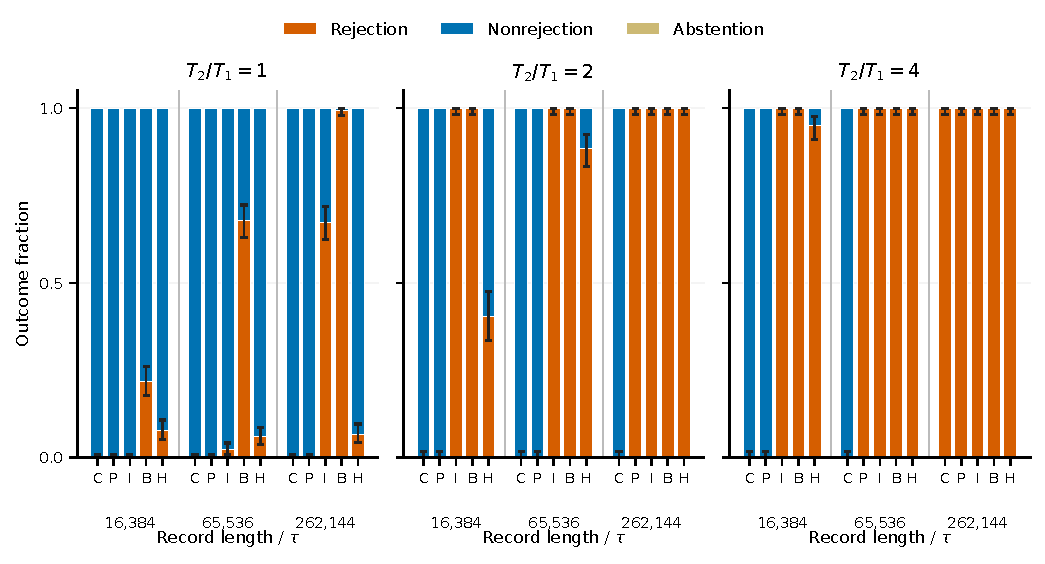
\includegraphics[width=\textwidth]{figures/brownian_operating_compact.pdf}
\caption{Raw bootstrap detections reach $397/400$ at equilibrium, while the calibrated source test rejects $0/400$. Temperature ratios are 1, 2, and 4; lengths are $N/2$ relaxation times. Methods: C, calibrated; P, phase ignored; I, independent windows; B, moving-block bootstrap; H, imaginary coherency. Equilibrium cells have 400 records; alternatives have 200. Bars give pointwise 95\% binomial intervals. Raw methods test recorded asymmetry; C tests source reversibility under response information. No method abstains. Values are saved study results.}\label{fig:study-brownian}
\end{figure*}

\begin{table*}[t]
\caption{Comparison targets. An approximate test for recorded asymmetry is not a finite-sample test for source reversibility under unequal sensors.}\label{tab:comparators}
\begin{ruledtabular}\begin{tabular}{>{\raggedright\arraybackslash}p{.20\textwidth}>{\raggedright\arraybackslash}p{.32\textwidth}>{\raggedright\arraybackslash}p{.19\textwidth}>{\raggedright\arraybackslash}p{.20\textwidth}}
Procedure & Null restriction & Detector information & Guarantee here\\
Calibrated contrast & Reversible source within the allowed response model & Relative phase and full covariance bound & Finite false-rejection bound\\
Spectral cycle & Real source cross spectra under sampled diagonal responses & Factorization; covariance and tail bounds & Finite false-rejection bound\\
Independent-window lag rule & Zero recorded lag contrast & None & Ignores overlapping-window dependence\\
Moving-block bootstrap & Zero recorded lag contrast & None in raw form & Approximate bootstrap\\
Imaginary coherency & Zero imaginary normalized cross spectrum & None & Approximate segment bootstrap\\
Phase-adjusted comparators & Recorded contrast within a detector allowance & Same phase bound as calibrated rule & No finite source-null guarantee here\\
\end{tabular}\end{ruledtabular}
\end{table*}
Table~\ref{tab:comparators} states the comparison targets before interpreting their rejection fractions. SM Secs.~S8.5 and S9.4 give their definitions and the phase-boundary controls.

\section{Three channels without phase calibration}\label{sec:main-cycle}
A third channel offers a way to remove detector phase without measuring it. Compare channels one and two, then two and three, then three and one. Each detector's timing shift enters twice, with opposite signs, and cancels around this triangle. Radio interferometry uses the same cancellation between measurements from pairs of antennas~\cite{jennison1958,thyagarajan2022}. Two channels are insufficient because $F_{12}F_{21}=|F_{12}|^2$ is always real. With three channels, the product can retain source phase after the detector phases cancel.

Let $F_{ij}(\omega)$ be the observed cross-spectral density and $S_{ij}(\omega)$ the source density. Their complex phases describe relative timing at frequency $\omega$. Here the densities refer to the absolutely continuous parts of the spectral measures. Population identities hold almost everywhere. The finite test below uses continuous observed cross spectra, supplied by absolute summability. In the sampled observation model,
\begin{equation}
 F_{12}F_{23}F_{31}=|H_1H_2H_3|^2 S_{12}S_{23}S_{31}.
 \label{eq:main-cycle-cancel}
\end{equation}
The detector factor on the right is real and nonnegative. Any imaginary part, the component that changes sign on reversal, must therefore come from the source product. Define
\begin{equation}
 J(\omega)=\operatorname{Im}\{F_{12}(\omega)F_{23}(\omega)F_{31}(\omega)\}.
 \label{eq:main-cycle}
\end{equation}
A reversible Gaussian source has real cross spectra, so $J=0$ almost everywhere. Under the continuity condition below, this equality holds at each tested frequency. A nonzero value rules out that source explanation under the response model. A zero value does not prove reversibility, because source asymmetry can cancel too. For pure delays, the phase contributions sum to $-\omega[(d_1-d_2)+(d_2-d_3)+(d_3-d_1)]=0$. Figure~\ref{fig:mechanism} contrasts this cancellation with a calibrated allowance. The identity concerns the full observed spectrum, which a finite record does not determine. The finite-law ambiguity therefore remains until further information controls the covariance at both observed and unobserved lags.

\subsection{Uncertainty on the three spectral edges}
To estimate the cycle, we use covariances only up to a chosen time separation, the lag cutoff. The error has two sources. Covariances estimated from the record fluctuate, and omitted lags can change the population spectrum. Assume absolute summability of the three observed cross-covariance sequences: their absolute values have a finite sum. Fix a lag cutoff $0\le L<N$ and $G$ frequencies before observation. Supply positive $K_i$ and nonnegative $B_{ij}$ such that
\begin{align}
 \Gamma_N&\preceq D_K,\label{eq:cycle-diagonal}\\
 \sum_{|k|>L}|C_{ij}(k)|+
 \frac1N\sum_{|k|\le L}|k|\,|C_{ij}(k)|&\le B_{ij},
\label{eq:main-cycle-tail}
\end{align}
Here $D_K=\operatorname{diag}(K_iI_N)_{i=1}^3$. The second condition holds for $ij\in\{12,23,31\}$. Equation~\eqref{eq:cycle-diagonal} is a bound for the full covariance matrix. Separate marginal bounds do not imply it. The bias allowance in Eq.~\eqref{eq:main-cycle-tail} covers the unobserved covariance tail and the finite lag weights.

Set $P_N=I-\mathbf1\mathbf1^{\mathsf T}/N$, $h=2L+1$, and
\[
 \begin{gathered}
 [W_\omega]_{st}=\mathbf1\{|s-t|\le L\}e^{-i\omega(s-t)},\\
 \widehat F_{ij}=N^{-1}(P_Ny_i)^{\mathsf T}W_\omega(P_Ny_j).
 \end{gathered}
\]
Each channel pair is an edge of the spectral triangle. An edge radius bounds the error in its estimated cross spectrum. For error probability $\delta_{\rm e}$ and $t_\delta=\log(12G/\delta_{\rm e})$, simultaneous edge radii are
\begin{equation}
 e_{ij,\delta}=B_{ij}+\sqrt{K_iK_j}
 \left(\frac{3h}{N}+2\sqrt{\frac{ht_\delta}{N}}
                  +\frac{\sqrt2 ht_\delta}{N}\right).
 \label{eq:main-cycle-radius}
\end{equation}
The allowance $B_{ij}$ covers the covariance truncation and finite lag weights. The $3h/N$ term covers centering, and the remaining terms cover sampling fluctuations. Increasing the cutoff retains more covariances and reduces the omitted tail, but it also increases $h$ in the sampling terms. The fixed cutoff must therefore be assessed through the complete radius. These edge errors must be propagated through the product before a nonzero estimated cycle can support rejection. For $x=(|\widehat F_{12}|,|\widehat F_{23}|,|\widehat F_{31}|)$ and the corresponding $e=(e_{12},e_{23},e_{31})$, define
\begin{equation}
 \mathcal R_\times(x,e)=\prod_{j=1}^3(x_j+e_j)-\prod_{j=1}^3x_j.
 \label{eq:cycle-product-radius}
\end{equation}
This is the sum of all seven terms that contain at least one edge error. The logarithm covers six real components, two tails, and $G$ frequencies at total error $\delta_{\rm e}$.

\begin{theorem}[Cycle test]\label{thm:main-cycle-test}
Under the sampled stationary Gaussian reversible-source model and Eqs.~\eqref{eq:cycle-diagonal}--\eqref{eq:main-cycle-tail}, reject if at least one of the $G$ fixed frequencies satisfies
\begin{equation}
 |\operatorname{Im}(\widehat F_{12}\widehat F_{23}\widehat F_{31})|
      >\mathcal R_\times(x,e_\alpha).\label{eq:main-cycle-test}
\end{equation}
The rejection probability is at most $\alpha$. Equality does not reject.
\end{theorem}

In words, reject when the estimated loop's imaginary part exceeds the largest change that the allowed estimation errors could produce. The proof normalizes channel $i$ by $\sqrt{K_i}$, applies Gaussian bounds to every pairwise spectrum, and expands the product error. This covers overlapping samples and the fixed frequency set (SM Sec.~S4.2, Theorem~S5). Deterministic recording errors enlarge each edge radius as described in SM Sec.~S4.3.

\subsection{What the cycle preserves and what it cannot identify}
The separate edge radii allow the rule to respect different channel scales. The rule is unchanged by an invertible change of channel units when every bound undergoes the corresponding transformation. Under $z_i\mapsto a_i z_i+b_i$, $a_i\ne0$, use $K_i\mapsto a_i^2K_i$, $B_{ij}\mapsto|a_ia_j|B_{ij}$, and $\eta_i\mapsto|a_i|\eta_i$. The statistic and threshold both multiply by $(a_1a_2a_3)^2$. This invariance changes data and all bounds together. Reducing signal gain while keeping added noise fixed changes the signal-to-noise ratio and is a different experiment. Response zeros can erase the witness, and numerical limits can still prevent a decision.

At one frequency, channel phases can make all cross spectra real exactly when every product around a cycle of nonzero edges is real. One proves this by first making the edges of a spanning tree positive. A spanning tree connects all channels without a cycle. Each remaining edge closes a cycle. For a Markov chain, the Kolmogorov criterion equates the products of forward and reverse transition rates around every loop~\cite{kelly1979}. Here the products contain complex cross spectra rather than nonnegative rates. Spectral products can be negative real, and the condition does not construct causal responses across frequencies. A real cycle is compatible with reversibility but also with sources whose asymmetry this frequency does not reveal.

The full covariance ceiling remains necessary for this finite-window argument even when it is conservative. Replacing it by only the spectral value at the tested frequency is invalid under these assumptions. For independent channels $Y_i(t)=Z_i(t)+Z_i(t-2)$, each spectrum vanishes at $\pi/2$, but a finite cross-spectral estimate has positive variance there. A finite window mixes nearby frequencies. SM Secs.~S4.2--S4.3 give this counterexample, the gain result, and a sufficient power condition.

\begin{figure*}[t]\centering
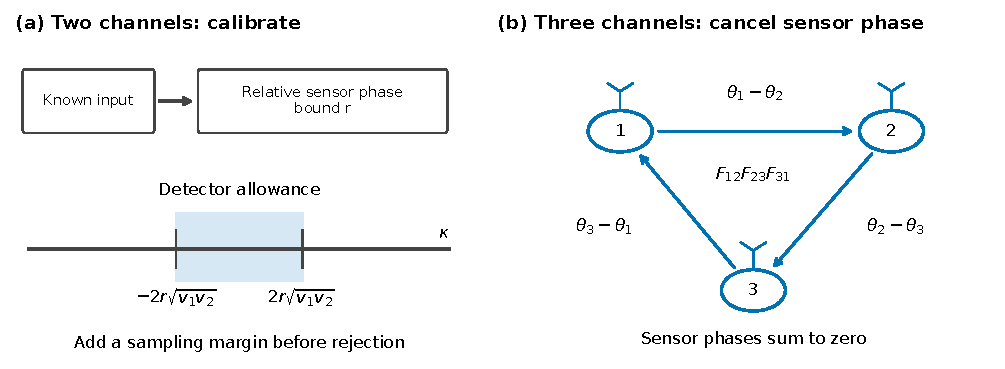
\includegraphics[width=\textwidth]{figures/mechanism_compact.pdf}
\caption{Calibration bounds detector phase, while a three-channel closure product cancels it. The calibrated route allows a nonzero source-null lag contrast and adds a sampling margin. The cycle route uses the three oriented cross spectra; each channel phase appears once with each sign. Both routes still require a full covariance bound. The spectral route also needs a bound on omitted lags.}\label{fig:mechanism}
\end{figure*}

\subsection{A rotating source and the cost of the edge bounds}
Finite detection also requires spectral estimates accurate enough to reveal source motion. We use a three-dimensional version of the trapped-particle model. Random motion relaxes toward the center while a rotational force circulates it about the $(1,1,1)$ axis. The model has
\begin{equation}
 A=\lambda I+\Omega,\quad D=\lambda\Sigma_\xi,\quad
 \Omega=\nu\begin{pmatrix}0&-1&1\\1&0&-1\\-1&1&0\end{pmatrix},
\end{equation}
where $\Sigma_\xi=(1-\xi)I+\xi\mathbf1\mathbf1^{\mathsf T}$. For $\lambda=\log4$ and $\nu=2\pi/(3\sqrt3)$, one sampling interval gives a $2\pi/3$ rotation and a cyclic coordinate permutation, attenuated by $1/4$. The equilibrium control sets $\nu=0$. Both use $\xi=1/4$ and the same family bounds.

Over $0\le\xi\le1/4$ and $\lambda\ge\log4$, the source spectral ceiling is $5/2$. If $g_i$ is the absolute sum of detector coefficients, valid diagonal ceilings are $K_i=(5/2)g_i^2$. Geometric covariance decay also gives the tail allowances at $L=8$ (SM Sec.~S7.3). The filters have principal delays zero, one, and two samples, with small later echoes. These bounds apply to the complete covariance; they are not three independent marginal assertions.

Figure~\ref{fig:study-cycle} shows when these allowances permit rejection. At $N=1048576$, the common and diagonal single-frequency rules each reject $1/200$ rotating records; the two-frequency rule rejects $200/200$. All three reach $200/200$ at $N=2097152$, while equilibrium controls give no rejections. The gain comparison in SM Fig.~S3 explains why diagonal bounds matter: they preserve all $200/200$ rejections across the six transported gains, while a common scalar ceiling loses them at four gains. Valid covariance inflation can also remove detection (SM Fig.~S4).

\begin{figure*}[t]\centering
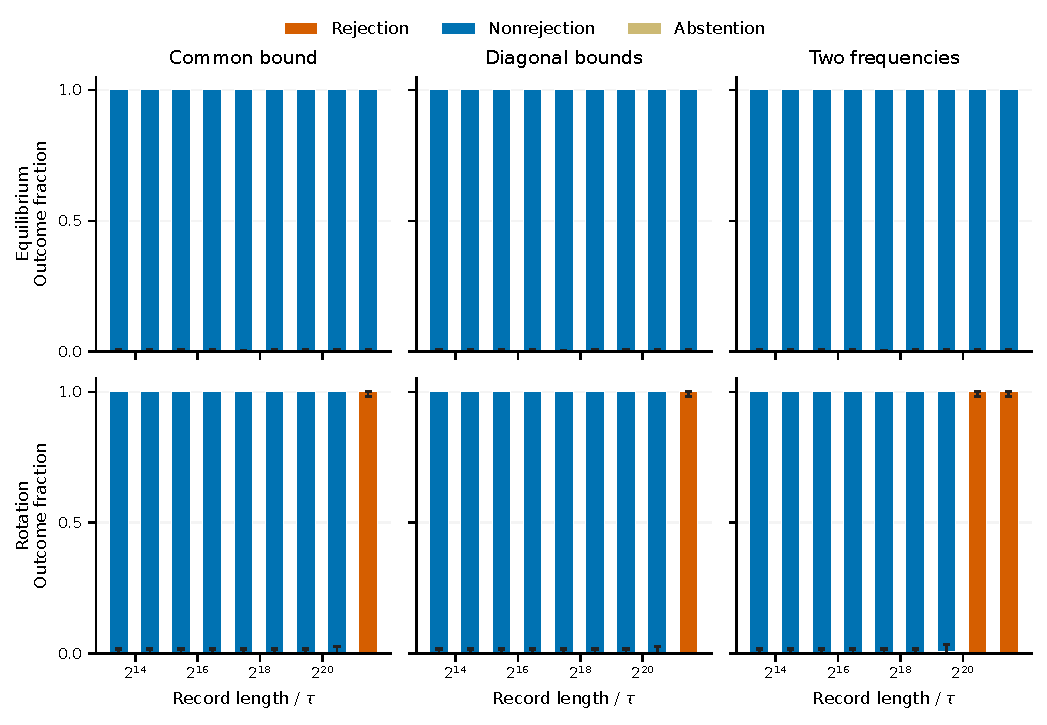
\includegraphics[width=\textwidth]{figures/cycle_operating_compact.pdf}
\caption{The two-frequency rule detects rotation at a shorter tested length than either single-frequency rule. Lengths are shown as $N\log4$ decay times. Fractions use all 200 rotating records per length; equilibrium cells have 400, except 1000 at $N=131072$. Bars are pointwise 95\% binomial intervals. The two-frequency error allowance is included. Common and diagonal decisions coincide in this primary comparison. All methods have zero abstentions. These empirical fractions do not replace the sufficient power condition.}\label{fig:study-cycle}
\end{figure*}

\section{How much data does inference require?}\label{sec:cost}
Even with perfect detector knowledge, dependence can leave a short record uninformative. Correlated samples can repeat nearly the same information, so an informative frequency band may require a long record. We first remove calibration and source-fitting uncertainty to isolate the recording cost imposed by the source itself.

Consider unit-variance Gaussian channels with identity responses, so the sensors leave the source unchanged. Their marginal spectral densities lie between $1/2$ and $\mathcal S/2$. The spectral dynamic range $\mathcal S\ge3$ measures the ceiling relative to the floor. We seek an absolute covariance contrast at least $\gamma$, with $0<\gamma\le1/4$. A difficult alternative places its directional signal in two narrow frequency bands. A length-$N$ record resolves only about $N/(\mathcal S-1)$ directions in those bands. Many samples then carry little new evidence about the asymmetry. Relative entropy measures how distinguishable this record's probability law is from a reversible law and therefore limits every test. The same information measure relates forward and reversed trajectories to dissipation in stochastic thermodynamics~\cite{roldan2010,seifert2012}.

\begin{theorem}[Recording cost]\label{thm:main-cost}
For each $(\mathcal S,\gamma)$ in this class, SM Sec.~S6 constructs a fixed reversible source and a fixed alternative with contrast $-\gamma$ and the same known marginal spectra. The necessary length inequality in SM Sec.~S6.3 applies to any test of this pair with false-rejection probability $\alpha$ and detection probability $1-\beta$, where $0<\alpha,\beta<1$ and $\alpha+\beta<1$. For the full class, the calibrated test with exact identity responses and $q=\mathcal S$ has false-rejection probability at most $0.05$ and detection probability at least $0.95$ whenever
\begin{equation}
 N\ge1024\mathcal S/\gamma^2.\label{eq:cost-uniform}
\end{equation}
At $\mathcal S=9$, $\gamma=0.1$, and $\alpha=\beta=0.05$, at least $5214$ samples are necessary for the fixed pair; direct evaluation of the sharper sufficient condition gives $129580$ samples for the full class.
\end{theorem}
Thus dependence can force thousands of samples even with exact responses. SM Sec.~S6, Theorems~S8--S9, gives the complete necessary inequality, its finite trace-defect bound, and the sufficient calculation. The information required by the two error rates is $(1-\beta)\log[(1-\beta)/\alpha]+\beta\log[\beta/(1-\alpha)]$. A record is necessarily too short if an upper bound on its available relative entropy is smaller. The sufficient-to-necessary length ratio is below $25$ in the worked case. It compares a class-wide sufficient bound with a fixed-pair lower bound, so it is not an optimal-length claim.

\subsection{Unknown persistence: why the whole confidence set matters}\label{src16:main}
Persistence describes how strongly a source value remains related to later values. When this dependence is unknown, the test must bound how much remains after filtering. Assume a noiseless single-channel reference from a stationary Gaussian first-order autoregression, or AR(1). A centered value equals $\phi$ times its predecessor plus an independent Gaussian innovation, the new random input at that step. For $0<\phi<1$, its decay time is $-1/\log\phi\simeq1/(1-\phi)$ samples near one. Thus $(N-1)(1-\phi)$ measures record length in approximate correlation times. At $\phi=0.995$, the lengths $16385$, $32769$, and $524289$ span about $82$, $164$, and $2621$ such times.

If $\phi$ were known, the common filter $(-\phi,1)$ would remove autoregressive spectral variation. This filter subtracts the predicted part of each value and uses the same operation on both channels, leaving relative detector phase unchanged. With unknown persistence, a single fitted value cannot guarantee the required bound. We instead retain a confidence set of candidate values that are compatible with the record under a specified test. For each candidate, we compare cumulative prediction errors with their finite Gaussian distribution. The resulting two-sided set has coverage at least $0.995$: over repeated recordings, it contains the true persistence with at least this probability. Its construction, exact law, and conservative numerical cutoffs are in SM Secs.~S5.1--S5.3.

To transfer this set to the pair, both Gaussian source marginals must have the same persistence. The reference response is a nonzero scalar, the second response is a nonzero finite impulse response, and both channels are noiseless before bounded recording. Their cross spectrum is arbitrary subject to positivity and is real under the null. Independent calibration covers the unchanged second response. These assumptions connect reference information to both testing channels.

Let $[\ell,u]$ be the smallest interval containing all accepted persistence values, called the confidence hull. For $u<1$, define $\Lambda(x)=(1+x)/(1-x)$ and $z(x)=\log\Lambda(x)$. The AR(1) spectral maximum-to-minimum ratio is $\Lambda(\phi)^2$, so this transform measures the spectral variation that the covariance bound must cover. For a fixed common-filter coefficient $a$,
\begin{equation}\label{src16:placement}
 \mathcal S_a=\exp\{z(u)-z(\ell)+2|z(a)-z_c|\},\quad
 z_c=\tfrac12[z(u)+z(\ell)].
\end{equation}
The first term is uncertainty in the source. The second is the cost of placing a fixed filter away from the interval's transformed center. A wide confidence set therefore creates a large threshold even when it covers the truth and excludes one.

Let $\alpha_B$ be the source-set error, $\alpha_L$ an additional lag-set error, and $\beta$ the common energy-event failure probability.
\begin{theorem}[Source-envelope consequence]\label{src16:envelope-thm}
Assume the two-sided source set and common energy event specified in SM Sec.~S5.4, under the positive-denominator conditions stated there. On source coverage and that event, the confidence hull is nonempty, $u<1$, and
\begin{equation}\label{src16:span}
 \frac{\Lambda(u)}{\Lambda(\ell)}\le2C_{\rm gap}.
\end{equation}
The constant $C_{\rm gap}$ is explicit in the full statement in SM Sec.~S5. The probability is at least $1-\alpha_B-\beta$, or $1-\alpha_B-\alpha_L-\beta$ for the lag intersection.
\end{theorem}
In words, the stated bounds on squared fluctuations control every accepted persistence value, even if the confidence set has separate pieces. Persistence values close to one allow very slow decay and therefore large covariance bounds. Excluding one by itself only makes the envelope finite; the additional inequalities control its size. SM Secs.~S5.4--S5.5 prove the result and its correlation-time scaling. At persistence $0.8$, a target probability $0.75$ of a nonempty set excluding one requires at least $65$ differences, while $256$ suffice under error allowance $0.005$ (SM Sec.~S5.7). This factor-of-four bracket concerns endpoint exclusion, not rejection.

The test uses a finite list of filters fixed before observation. For $M$ members, the source, calibration, variance, and contrast allocations in Table~\ref{tab:budget} cover the complete union decision. A length-dependent list $a_j=1-2^{-j}$ controls placement near persistence one, whereas a fixed list bounded away from one cannot do so uniformly. SM Sec.~S5.8 gives the rule, including empty sets and unavailable members.

\subsection{A complete detection example and its observed limits}
To establish sensitivity, the preceding bounds must jointly permit rejection. The example below combines source estimation, calibration, and finite arithmetic to bound detection probability at one specified long length. Its shorter-length failures show where the same sufficient conditions remain uninformative.

\paragraph{Example: a delayed persistent source.}\label{src16:power-thm}
Let $X,Z$ be independent unit-variance Gaussian AR(1) processes with $\phi=0.995$. Observe
\[
 Y_1(t)=2+X_t,\qquad
 Y_2(t)=-1+0.9X_{t-1}+\sqrt{0.19}Z_t.
\]
Use identity responses, $N=524289$, independent 256-row two-coefficient calibration with noise standard deviation $0.01$, and the bank $(0,0.5,0.8,0.9,0.97,0.995)$. Values lie on the $2^{-20}$ grid within $2^{-21}$ of the ideal samples. Under the complete design and bounded arithmetic specified in SM Secs.~S5.9--S5.10,
\begin{equation}\label{src16:implemented-power}
 \Pr(\mathrm{reject})\ge0.91-(4N+512)e^{-128}>0.90.
\end{equation}
The full parameter statement is retained in SM Sec.~S5. The bound includes completion of all calculations needed for rejection. Earlier points on the doubling grid fail a source, variance, or contrast-margin condition; the long-record result gives no corresponding shorter-record guarantee.

The saved synthetic comparison shows how these requirements affect decisions (Fig.~\ref{fig:study-source}). Table~\ref{tab:source-outcomes} shows the transition from unavailable or inconclusive tests to detection. The lag set abstains throughout the two shorter cells because its upper endpoint still reaches one. SM Fig.~S7 locates the first failed condition, and Figs.~S1--S2 and S8 separate coverage from endpoint availability.

The improvement is conditional. At $N=8193$, the standalone set rejects $46/200$ and its split-budget intersection rejects $32/200$. Their paired difference is $0.070$, with conservative 95\% interval $[-0.006,0.142]$. At moderate persistence the intersection can instead retain detections lost by the standalone set. The two-sided threshold diagnostics at $N=524289$ have median phase allowance about $7.6\times10^{-5}$ and median sampling radius about $5.0\times10^{-4}$ (SM Figs.~S5--S6). These saved summaries show that estimating dependence remains costly even when phase calibration is accurate.

\begin{figure*}[t]\centering
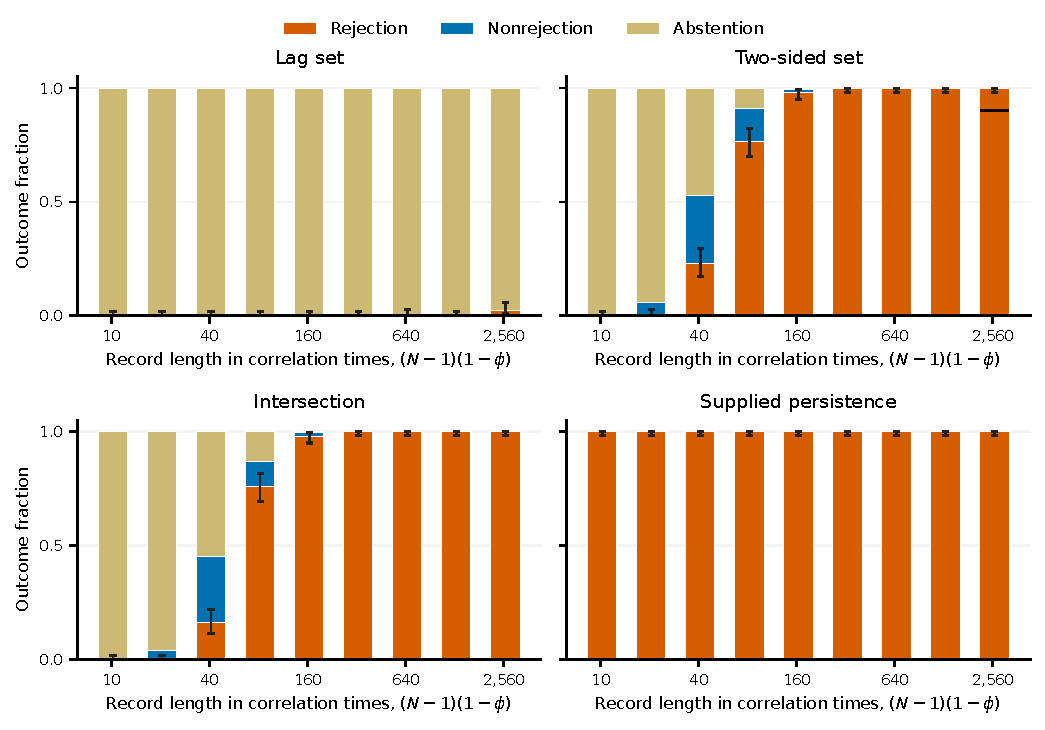
\includegraphics[width=\textwidth]{figures/source_operating_compact.pdf}
\caption{Estimating persistence delays detection even when the supplied-persistence test rejects every alternative record. Outcomes are shown against approximate correlation times $(N-1)(1-\phi)$ at $\phi=0.995$, with 200 independent records per length. Lag confidence often reaches persistence one and therefore causes abstention. Two-sided confidence becomes useful sooner; intersection is not uniformly better. Rejection intervals are pointwise 95\% binomial intervals. The ideal-model lower bound at the longest length is distinct from the observed fraction.}\label{fig:study-source}
\end{figure*}

\begin{table}[t]
\caption{Two-sided source inference at $\phi=0.995$ and strong delay. Each row uses 200 independent records. R, NR, and A denote rejection, nonrejection, and abstention.}\label{tab:source-outcomes}
\begin{ruledtabular}\begin{tabular}{rrrrr}
$N$ & $(N-1)(1-\phi)$ & R & NR & A\\
16385 & 81.92 &153&29&18\\
32769 &163.84&196&3&1\\
524289&2621.44&200&0&0\\
\end{tabular}\end{ruledtabular}
\end{table}

\section{What sampling hides}\label{sec:sampling}
The preceding tests attribute asymmetry to the sampled source. To relate that conclusion to thermodynamics, one must also account for motion between observations. The rotating model makes this remaining ambiguity explicit. Adding a full turn between samples changes the continuous motion without changing the observed transition.

Set $\nu=2\pi/\sqrt3$ in the model of Sec.~\ref{sec:main-cycle}. Rotation then completes a full turn per sample, and the transition is $I/4$. The sampled Gaussian source is reversible although its continuous-time probability current is nonzero. The detector-phase cancellation remains valid, but it cannot restore time order absent from the source samples.

For this reason, the entropy-production rate requires the continuous-time dynamics, not only their sampled law. For overdamped coordinates with even reversal parity, the stationary rate is~\cite{seifert2012}
\begin{equation}
 \sigma=\operatorname{tr}\{(A-D\Sigma^{-1})^{\mathsf T}
 D^{-1}(A-D\Sigma^{-1})\Sigma\}.
\end{equation}
It measures irreversibility in units of $k_B$ per unit time and vanishes at detailed balance for these models. The rotational rate is $6\nu^2/\lambda$. More generally,
\begin{equation}
 \nu_k=(2\pi/3+2\pi k)/\sqrt3,\qquad k\in\mathbb Z,
\end{equation}
gives the same sampled transition and innovation covariance for every integer $k$, while $6\nu_k^2/\lambda$ grows without bound. SM Sec.~S7.4 derives both the aliasing identity and the entropy rates. Thus even complete knowledge of the sampled law cannot determine continuous-time entropy production without additional dynamical or bandwidth information.


\section{Discussion}
A recorded direction in time can belong to the source, the detectors, or both. Calibration limits the detector contribution, while closure phase cancels it under a sampled diagonal response model. Neither operation removes sampling uncertainty or restores motion hidden between samples.

For an experiment, first establish which response model describes the acquired sequence. With two channels, use a known input to bound their relative phase. With three or more channels, closure phase can avoid this calibration only when each response acts on its own sampled source channel and detector errors are uncorrelated between channels. Control bandwidth or justify the treatment of aliases. Then obtain a full covariance bound from physical dynamics or a valid source-confidence procedure, together with a covariance-tail allowance for the spectral test. Evaluate the resulting threshold before interpreting a nonzero signal. Record length in correlation times is a useful starting point, but conservative family bounds can require much more data, as the Brownian example shows.

The tests connect established operations to a specific source null. Closure products remove local phase~\cite{thyagarajan2022}; Gaussian quadratic-form bounds control dependent estimates~\cite{laurentmassart,hsukakadezhang,basumichailidis}; and exact autoregressive inversion supplies confidence sets~\cite{dufour1990,dufourking1991,andrews1993}. Here these operations must preserve a nonzero detector allowance, cover the whole fitted source set, and reach a finite-record decision. Coverage alone is insufficient if a confidence set leaves the threshold uninformative. The two-sided construction improves several persistent conditions, but its intersection with lag confidence changes rejection in both directions because the component error allocations also change.

Different null hypotheses require different interpretations. Bi and Calhoun use a coherence witness for shared hidden input~\cite{bicalhoun2026}. Their multiplicative response model filters independent noise and shared input together, allowing response factors to cancel. Their null has independent probes; ours permits correlated reversible sources. Raw lag and imaginary-coherency procedures instead test recorded-signal asymmetry. Their equilibrium detections under unequal responses are evidence against that recorded-signal null, not contradictions of the calibrated source guarantee. The near-boundary controls make the distinction especially clear: raw procedures reject all $400$ records, while calibrated procedures reject none, even when detector-induced contrast reaches $99\%$ of its population tolerance (SM Sec.~S9.4).

Detector control also leaves a distinct thermodynamic question. Relative entropy between forward and reversed trajectories constrains dissipation when the observation and dynamics satisfy the required assumptions~\cite{seifert2012,lucenteinference2022,ohgaasymmetry2023}. In the rotational example, different continuous dynamics have the same sampled law and arbitrarily different entropy-production rates. A closure product cannot recover that missing temporal information. Detector-aware bounds on entropy production will therefore need additional bandwidth or dynamical constraints.

The guarantees assume stationarity, joint Gaussian laws, stable linear responses, fixed channel identities and common reversal parity, and the specified covariance and error bounds. Source fitting additionally requires a noiseless scalar reference and shared autoregressive marginal persistence. Reference noise, non-Gaussian innovations, correlated detector errors, and underestimated bounds lie outside the corresponding guarantees. The sensitivity results describe only the tested conditions, and all physical examples are synthetic. Bounded recording corrections cover a valid rounding error; they do not make a finite random generator exactly Gaussian. Extensions to non-Gaussian sources, nonlinear responses, and detector-aware entropy bounds remain open. Within the present model, the tests state when unequal sensors and sampling uncertainty no longer suffice to explain the observed asymmetry.

\appendix
\section{Methods}\label{sec:study-methods}
The observation filters, alignment anchors, tested contrasts, frequency sets, model families, sample counts, and analysis rules were fixed before the records for the present study were generated. No method or parameter was selected from the outcomes of the present study. The study has $69$ conditions and $20800$ independent records. Paired transformations and numerical settings do not add independent records.

The source pair is $X_1(t)=X(t)$ and $X_2(t)=cX(t-d)+\sqrt{1-c^2}Z(t)$, where $X,Z$ are independent stationary unit-variance Gaussian AR(1) processes. The null has $(d,c)=(0,0.9)$; the alternatives have $(1,0.4)$ and $(1,0.9)$. Recording means are $2,-1$. The principal detector responses are identities. A separate $256$-row calibration fits two coefficients using orthogonal sign columns and independent mean-zero Gaussian errors of standard deviation $0.01$. Both coefficients are fitted when one true coefficient is zero. The primary fixed bank is $(0,0.5,0.8,0.9,0.97,0.995)$. A separately declared bank uses $1-2^{-j}$ through $j=\lceil\log_2(N-1)\rceil$.

The calculations use exact recorded moments and arithmetic bounds that enclose each result conservatively. Unresolved comparisons cause abstention; unexpected execution failures remain separate. SM Sec.~S8.6 gives the precision settings and work limits.

The principal recordings have $20$ fractional bits and include the corresponding bounded-error correction. Paired grids with $8$ and $12$ fractional bits isolate rounding. Separate finite $8$-bit and $12$-bit recorders span $[-16,16)$, with clipping to the outer bin centers. Saturation without a valid perturbation certificate causes abstention. Calibration stays at the primary recording precision in these comparisons.

The moving-block bootstrap~\cite{kunsch1989} uses $499$ resamples and block length $\max\{2,\lceil n_b^{1/3}\rceil\}$ for the centered product sequence. Here $n_b=N-2$ is the retained product count after omitting row zero, as specified in SM Sec.~S8.5. Its probability estimate uses a plus-one correction. Imaginary coherency~\cite{noltecoherency2004} uses nonoverlapping $256$-sample segments at frequency $\pi/2$ and the declared bootstrap of segment contributions. An incomplete final segment is omitted only for this comparator. Missing phase information causes the phase-adjusted comparators to abstain.

Each cell has a pointwise two-sided $95\%$ Clopper--Pearson confidence interval~\cite{clopper}. A paired rejection difference uses the two discordant outcomes. Subtracting simultaneous $97.5\%$ intervals for their probabilities gives a conservative $95\%$ difference interval. Each interval quantifies uncertainty in its own rejection probability or paired difference over repeated studies. These intervals are pairwise, without a familywise guarantee across all comparisons. Rejection among available tests and threshold quantiles are descriptive. Exact rational comparisons determine source-set coverage and whether its upper endpoint is below one before numerical summaries are formed.

The recorded study environment uses Python 3.9.6, NumPy 2.0.2, SciPy 1.13.1, and Matplotlib 3.9.4~\cite{harris2020numpy,virtanen2020scipy,hunter2007matplotlib}. Certified probability integrals used Python 3.12.14, NumPy 2.5.3, and python-flint 0.9.0. The package retains the certificates and environment files. Empirical fractions concern the declared finite generator; the mathematical power bound concerns the ideal Gaussian law followed by bounded recording.

\begin{table}[t]
\caption{Main notation. Source and recorded covariances are distinguished by the superscript $X$.}\label{tab:notation}
\begin{ruledtabular}\begin{tabular}{p{0.24\columnwidth}p{0.68\columnwidth}}
Symbol & Meaning \\
$N,n=N-1$ & Samples and adjacent pairs. \\
$F_{ij},S_{ij}$ & Recorded and source spectral densities. \\
$\kappa,r$ & Lag contrast and relative-phase bound. \\
$q,K_i$ & Full-record covariance bounds, standardized or channel scaled. \\
$L,B_{ij}$ & Retained lag cutoff and omitted-lag bias allowance. \\
$\phi,\psi,a_j$ & True persistence, candidate persistence, common-filter coefficient. \\
$\mathcal S_a,\Lambda(x)$ & Residual spectral ratio and $(1+x)/(1-x)$. \\
\end{tabular}\end{ruledtabular}
\end{table}

\subsection{Constructing the covariance envelope}\label{sec:covariance-construction}
One construction uses a source spectral floor and ceiling. If normalized source marginal densities obey $0<m_0\le g_i\le M_0$, define $\mathcal S=M_0/m_0$. If calibration bounds $\sup|H_i|^2/\|h_i\|_2^2$ by $\widehat C_i$, and the error spectra obey $f_{E,i}\le J_i\operatorname{Var}E_i$, then
\begin{equation}
 \widehat q=\max\{2\mathcal S\max_i\widehat C_i,\max_iJ_i\}
 \label{eq:main-q}
\end{equation}
is valid when the calibration confidence regions contain the true response coefficients. Here $h_i$ is the vector of response coefficients. The source ratio and the error bounds are supplied separately. Physical dynamics can also supply the full bound directly, as in Sec.~\ref{sec:physical}.

\subsection{Response calibration and error allocation}\label{sec:calibration-details}
\begin{table}[t]
\caption{Error allocations explain the logarithms in the thresholds. Each column totals $0.05$. The fitted-source bank has $M$ fixed filters.}\label{tab:budget}
\begin{ruledtabular}\begin{tabular}{lcc}
Component & Calibrated pair & Fitted-source bank\\
Source confidence & --- & $0.005$\\
Calibration & $0.01$ & $0.01$\\
Both variance ceilings & $0.01$ & $0.01$\\
Contrast & $0.03$ & $0.025$\\\hline
Variance logarithm & $\log(200)$ & $\log(200M)$\\
Contrast logarithm & $\log(2/0.03)$ & $\log(80M)$\\
\end{tabular}\end{ruledtabular}
\end{table}

Calibration uses known deterministic inputs and a full-rank response design at fixed integer coefficient positions. Errors are independent Gaussian values with a common positive variance within each channel, and residual degrees of freedom are positive. Responses must stay unchanged between calibration and testing. Coefficient confidence regions and derivative bounds between grid points give an all-frequency phase allowance (SM Secs.~S3.4--S3.5). Table~\ref{tab:budget} gives the total false-rejection budget. Bounded rounding is covered by enlarging the variance ceilings and adding a deterministic contrast error (SM Sec.~S4.5, Proposition~S7).

\subsection{Scientific timing}
The supplied-source results were selected for comparison after their outcomes were known. The cycle and cumulative-innovation methods were developed after lag-ratio outcomes were known. Diagnostics of source-envelope geometry and threshold components were selected after inspection of the corresponding four-method comparison. They summarize its saved confidence sets and thresholds without changing decisions. The two-sided method and the present study design were developed with that evidence available, then fixed before their own fresh records were generated. The studies were not externally preregistered.

\subsection{Use of generative AI}
OpenAI GPT-6, GPT-6.1, and Anthropic Claude Opus 5.5 assisted with research ideas, mathematical derivations, programming, simulation execution, analysis, drafting, figures, and editing. The author directed the research question, scope, and restrictions, and required retention of adverse outcomes. Verification used separate mathematical derivations, exact-arithmetic checks, software tests, primary-source checks, and comparisons with saved numerical outputs. The author supplied the study direction and author information. The mathematical and numerical checks included AI assistance.

\begin{acknowledgments}
This work was funded by Emergent Ventures.
\end{acknowledgments}
\section*{Conflict of interest}
The author declares no competing interests.
\section*{Data availability}
This study uses only synthetic data. Code, study settings, random-generator states, complete present-study decision tables, numerical cutoff certificates, and saved figure and table data are available at \url{https://github.com/dvgyl/time-reversal-inference}. The versioned archive is deposited at \href{https://doi.org/10.5281/zenodo.23223118}{doi:10.5281/zenodo.23223118}. The compact release omits the full raw trajectories and detailed per-record numerical files, which are retained locally. The code and settings support regeneration. Floating-point arrays can differ across software versions and platforms. The release supplies the recorded environment and checksums for the complete saved package.
\begin{thebibliography}{99}
\bibitem{gonzalezarea2019} \href{https://doi.org/10.1103/PhysRevE.99.022143}{Gonzalez, J. P., Neu, J. C. \& Teitsworth, S. W. Experimental metrics for detection of detailed balance violation. \emph{Physical Review E} \textbf{99}, 022143 (2019).}
\bibitem{ohgaasymmetry2023} \href{https://doi.org/10.1103/PhysRevLett.131.077101}{Ohga, N., Ito, S. \& Kolchinsky, A.
Thermodynamic Bound on the Asymmetry of Cross-Correlations.
\emph{Physical Review Letters} \textbf{131}, 077101 (2023).}
\bibitem{cerasolispectra2022} \href{https://doi.org/10.1103/PhysRevE.106.014137}{Cerasoli, S., Ciliberto, S., Marinari, E., Oshanin, G., Peliti, L. \& Rondoni, L.
Spectral fingerprints of nonequilibrium dynamics: The case of a Brownian gyrator.
\emph{Physical Review E} \textbf{106}, 014137 (2022).}
\bibitem{seara} \href{https://doi.org/10.1038/s41467-020-20281-2}{Seara, D. S., Machta, B. B. \& Murrell, M. P. Irreversibility in dynamical phases and transitions. \emph{Nat. Commun.} \textbf{12}, 392 (2021).}
\bibitem{tongzhang} \href{https://www3.stat.sinica.edu.tw/statistica/oldpdf/A15n210.pdf}{Tong, H. \& Zhang, Z. On time-reversibility of multivariate linear processes. \emph{Statistica Sinica} \textbf{15}, 495--504 (2005).}
\bibitem{bhandari2026} \href{https://arxiv.org/abs/2608.13431v1}{Bhandari, A. Measuring the Arrow of Time: Identification, Estimation, and Inference for Directional Structure in Multivariate Time Series. Preprint, arXiv:2608.13431v1 (2026).}
\bibitem{stehbens2012} \href{https://doi.org/10.1016/B978-0-12-391857-4.00015-X}{S. Stehbens, H. Pemble, L. Murrow, and T. Wittmann, Imaging intracellular protein dynamics by spinning disk confocal microscopy, \emph{Methods in Enzymology} \textbf{504}, 293--313 (2012).}
\bibitem{bergsorensen2004} \href{https://doi.org/10.1063/1.1645654}{K. Berg-S\o rensen and H. Flyvbjerg, Power spectrum analysis for optical tweezers, \emph{Review of Scientific Instruments} \textbf{75}, 594--612 (2004).}
\bibitem{battle2016} \href{https://doi.org/10.1126/science.aac8167}{C. Battle, C. P. Broedersz, N. Fakhri, V. F. Geyer, J. Howard, C. F. Schmidt, and F. C. MacKintosh, Broken detailed balance at mesoscopic scales in active biological systems, \emph{Science} \textbf{352}, 604--607 (2016).}
\bibitem{gnesotto2018} \href{https://doi.org/10.1088/1361-6633/aab3ed}{F. S. Gnesotto, F. Mura, J. Gladrow, and C. P. Broedersz, Broken detailed balance and non-equilibrium dynamics in living systems: a review, \emph{Reports on Progress in Physics} \textbf{81}, 066601 (2018).}
\bibitem{seara2018} \href{https://doi.org/10.1038/s41467-018-07413-5}{D. S. Seara, V. Yadav, I. Linsmeier, A. P. Tabatabai, P. W. Oakes, S. M. A. Tabei, S. Banerjee, and M. P. Murrell, Entropy production rate is maximized in non-contractile actomyosin, \emph{Nature Communications} \textbf{9}, 4948 (2018).}
\bibitem{li2019} \href{https://doi.org/10.1038/s41467-019-09631-x}{J. Li, J. M. Horowitz, T. R. Gingrich, and N. Fakhri, Quantifying dissipation using fluctuating currents, \emph{Nature Communications} \textbf{10}, 1666 (2019).}
\bibitem{mura2018} \href{https://doi.org/10.1103/PhysRevLett.121.038002}{F. Mura, G. Gradziuk, and C. P. Broedersz, Nonequilibrium Scaling Behavior in Driven Soft Biological Assemblies, \emph{Physical Review Letters} \textbf{121}, 038002 (2018).}
\bibitem{gradziuk2019} \href{https://doi.org/10.1103/PhysRevE.99.052406}{G. Gradziuk, F. Mura, and C. P. Broedersz, Scaling behavior of nonequilibrium measures in internally driven elastic assemblies, \emph{Physical Review E} \textbf{99}, 052406 (2019).}
\bibitem{filliger2007} \href{https://doi.org/10.1103/PhysRevLett.99.230602}{R. Filliger and P. Reimann, Brownian gyrator: A minimal heat engine on the nanoscale, \emph{Physical Review Letters} \textbf{99}, 230602 (2007).}
\bibitem{argun2017} \href{https://doi.org/10.1103/PhysRevE.96.052106}{A. Argun, J. Soni, L. Dabelow, S. Bo, G. Pesce, R. Eichhorn, and G. Volpe, Experimental realization of a minimal microscopic heat engine, \emph{Physical Review E} \textbf{96}, 052106 (2017).}
\bibitem{hansenSargent1983} \href{https://doi.org/10.2307/1911996}{Hansen, L. P. \& Sargent, T. J. The dimensionality of the aliasing problem in models with rational spectral densities. \emph{Econometrica} \textbf{51}, 377--387 (1983).}
\bibitem{parratobar} \href{https://proceedings.neurips.cc/paper/2017/hash/333cb763facc6ce398ff83845f224d62-Abstract.html}{Parra, G. \& Tobar, F. Spectral mixture kernels for multi-output Gaussian processes. In \emph{Advances in Neural Information Processing Systems} \textbf{30} (2017).}
\bibitem{rutten} \href{https://proceedings.neurips.cc/paper/2020/hash/6d79e030371e47e6231337805a7a2685-Abstract.html}{Rutten, V. M. S., Bernacchia, A., Sahani, M. \& Hennequin, G. Non-reversible Gaussian processes for identifying latent dynamical structure in neural data. In \emph{Advances in Neural Information Processing Systems} \textbf{33} (2020).}
\bibitem{jennison1958} \href{https://doi.org/10.1093/mnras/118.3.276}{R. C. Jennison, A Phase Sensitive Interferometer Technique for the Measurement of the Fourier Transforms of Spatial Brightness Distributions of Small Angular Extent, \emph{Monthly Notices of the Royal Astronomical Society} \textbf{118}, 276--284 (1958).}
\bibitem{thyagarajan2022} \href{https://doi.org/10.1103/PhysRevD.105.043019}{Thyagarajan, N., Nityananda, R. \& Samuel, J. Invariants in co-polar interferometry: An Abelian gauge theory. \emph{Physical Review D} \textbf{105}, 043019 (2022).}
\bibitem{kelly1979} \href{https://www.statslab.cam.ac.uk/~fpk1/rsn.html}{F. P. Kelly, \emph{Reversibility and Stochastic Networks} (Wiley, Chichester, 1979), Chap. 1.}
\bibitem{roldan2010} \href{https://doi.org/10.1103/PhysRevLett.105.150607}{\'{E}. Rold\'{a}n and J. M. R. Parrondo, Estimating Dissipation from Single Stationary Trajectories, \emph{Physical Review Letters} \textbf{105}, 150607 (2010).}
\bibitem{seifert2012} \href{https://doi.org/10.1088/0034-4885/75/12/126001}{U. Seifert, Stochastic thermodynamics, fluctuation theorems and molecular machines, \emph{Reports on Progress in Physics} \textbf{75}, 126001 (2012).}
\bibitem{laurentmassart} \href{https://doi.org/10.1214/aos/1015957395}{Laurent, B. \& Massart, P. Adaptive estimation of a quadratic functional by model selection. \emph{Annals of Statistics} \textbf{28}, 1302--1338 (2000).}
\bibitem{hsukakadezhang} \href{https://arxiv.org/abs/1110.2842}{Hsu, D., Kakade, S. M. \& Zhang, T. A tail inequality for quadratic forms of subgaussian random vectors. \emph{arXiv} 1110.2842v1 (2011).}
\bibitem{basumichailidis} \href{https://doi.org/10.1214/15-AOS1315}{Basu, S. \& Michailidis, G. Regularized estimation in sparse high-dimensional time series models. \emph{Annals of Statistics} \textbf{43}, 1535--1567 (2015).}
\bibitem{dufour1990} \href{https://doi.org/10.2307/2938212}{Dufour, J.-M. Exact tests and confidence sets in linear regressions with autocorrelated errors. \emph{Econometrica} \textbf{58}, 475--494 (1990).}
\bibitem{dufourking1991} \href{https://doi.org/10.1016/0304-4076(91)90080-W}{Dufour, J.-M. \& King, M. L. Optimal invariant tests for the autocorrelation coefficient in linear regressions with stationary or nonstationary AR(1) errors. \emph{Journal of Econometrics} \textbf{47}, 115--143 (1991).}
\bibitem{andrews1993} \href{https://doi.org/10.2307/2951781}{Andrews, D. W. K. Exactly Median-Unbiased Estimation of First Order Autoregressive/Unit Root Models. \emph{Econometrica} \textbf{61}, 139--165 (1993).}
\bibitem{bicalhoun2026} \href{https://arxiv.org/abs/2604.03775v3}{Bi, Y. \& Calhoun, V. D. Cross-Spectral Witness for Hidden Nonequilibrium Beyond the Scalar Ceiling. Preprint, arXiv:2604.03775v3 (2026).}
\bibitem{lucenteinference2022} \href{https://doi.org/10.1103/PhysRevResearch.4.043103}{Lucente, D., Baldassarri, A., Puglisi, A., Vulpiani, A. \& Viale, M. Inference of time irreversibility from incomplete information: Linear systems and its pitfalls. \emph{Physical Review Research} \textbf{4}, 043103 (2022).}
\bibitem{kunsch1989} \href{https://doi.org/10.1214/aos/1176347265}{H. R. K\"unsch, The jackknife and the bootstrap for general stationary observations, \emph{Annals of Statistics} \textbf{17}, 1217--1241 (1989).}
\bibitem{noltecoherency2004} \href{https://doi.org/10.1016/j.clinph.2004.04.029}{Nolte, G., Bai, O., Wheaton, L., Mari, Z., Vorbach, S. \& Hallett, M.
Identifying true brain interaction from EEG data using the imaginary part of coherency.
\emph{Clinical Neurophysiology} \textbf{115}, 2292--2307 (2004).}
\bibitem{clopper} \href{https://doi.org/10.1093/biomet/26.4.404}{Clopper, C. J. \& Pearson, E. S. The use of confidence or fiducial limits illustrated in the case of the binomial. \emph{Biometrika} \textbf{26}, 404--413 (1934).}
\bibitem{harris2020numpy} \href{https://doi.org/10.1038/s41586-020-2649-2}{C. R. Harris \emph{et al.}, Array programming with NumPy, \emph{Nature} \textbf{585}, 357--362 (2020).}
\bibitem{virtanen2020scipy} \href{https://doi.org/10.1038/s41592-019-0686-2}{P. Virtanen \emph{et al.}, SciPy 1.0: Fundamental Algorithms for Scientific Computing in Python, \emph{Nature Methods} \textbf{17}, 261--272 (2020).}
\bibitem{hunter2007matplotlib} \href{https://doi.org/10.1109/MCSE.2007.55}{J. D. Hunter, Matplotlib: A 2D graphics environment, \emph{Computing in Science \& Engineering} \textbf{9}, 90--95 (2007).}
\end{thebibliography}

\end{document}
